\documentclass[a4paper]{article}
\usepackage{palatino}
\usepackage[english]{babel}
\usepackage{mathptmx}
\usepackage{flushend}
\usepackage{palatino}
\usepackage{enumitem}
\usepackage{wrapfig}
\RequirePackage{setspace,pdfpages,graphicx,color,geometry,hyperref,color,fancyhdr}
\geometry{tmargin=4.5cm}

% fancyhdr is only used to override the page numbering of the proposed table of contents (inside includepdf)
\fancyhf{} % sets both header and footer to nothing
\renewcommand{\headrulewidth}{0pt} % no horizontal line

% Default font
\RequirePackage[sc]{mathpazo}
\linespread{1.25}         % Palatino needs more leading (space between lines)
\RequirePackage[T1]{fontenc}

\title{\begin{onehalfspace}{\Huge Systemizing Glyph Design for Visualization}\end{onehalfspace}~\\ Report for Confirmation of Status}
\author{Eamonn James Maguire}
\date{April 2014}

\begin{document}
\maketitle\thispagestyle{empty}\clearpage\setcounter{page}{1}

\section*{Thesis abstract}
\newcommand{\ThesisAbstractDef}{[abstract]}
\newcommand{\ThesisAbstract}[1]{\renewcommand{\ThesisAbstractDef}{#1}}
\newcommand{\Abstract}{\ThesisAbstractDef}
\newcommand{\NOTETOSELFLONG}[1]{{\color{red}#1}}
\ThesisAbstract{%
The digitalisation of information now affects most fields of human activity.
From the social sciences to biology to physics, the volume, velocity, and variety of data exhibit exponential growth trends.
With such rates of expansion, efforts to understand and make sense of datasets of such scale, however driven and directed, progress only at an incremental pace.
The challenges are significant.
For instance, the ability to display an ever growing amount of data is physically and naturally bound by the dimensions of the average sized display.
A synergistic interplay between statistical analysis and visualisation approaches outlines a path for significant advances in the field of data exploration.
We can turn to statistics to provide principled guidance for prioritisation of information to display.
Using statistical results, and combining knowledge from the cognitive sciences, visual techniques can be used to highlight salient data attributes.

The purpose of this thesis is to explore the link between computer science, statistics, visualization, and the cognitive sciences, to define and develop more systematic approaches towards the design of glyphs.

Glyphs represent the variables of multivariate data records by mapping those variables to one or more visual channels (\eg, colour, shape, and texture).
They offer a unique, compact solution to the presentation of a large amount of multivariate information.
However, composing a meaningful, interpretable, and learnable glyph can pose a number of problems.
The first of these problems exist in the subjectivity involved in the process of data to visual channel mapping, and in the organisation of those visual channels to form the overall glyph.
Our first contribution outlines a computational technique to help systematise many of these otherwise subjective elements of the glyph design process.

For visual information compression, common patterns (motifs) in time series or graph data for example, may be replaced with more compact, visual representations.
Glyph-based techniques can provide such representations that can help users find common patterns more quickly, and at the same time, bring attention to anomalous areas of the data.
However, replacing any data with a glyph is not going to make tasks such as visual search easier.
A key problem is the selection of semantically meaningful motifs with the potential to compress large amounts of information.
A second contribution of this thesis is a computational process for systematic design of such glyph libraries and their subsequent glyphs.

A further problem in the glyph design process is in their evaluation.
Evaluation is typically a time-consuming, highly subjective process.
Moreover, domain experts are not always plentiful, therefore obtaining statistically significant evaluation results is often difficult.
A final contribution of this work is to investigate if there are areas of evaluation that can be performed  computationally.
}
\Abstract


\clearpage

\section*{Status of Research to Date}
At this point, the major body of my research in systemizing glyph design is complete. In the first year, much of my time was spent reading the literature on glyphs in general, and perception literature detailing how the human visual system works. This work was capped by a paper showing the first systematic way of creating glyphs and was presented at IEEE VisWeek in 2012 and published in IEEE TVCG \cite{Maguire:2012:TVCG}. 

In the second year, I contributed to a number of glyph papers including a survey of the domain \cite{Borgo:2013:EG} and a piece of work on the use of glyphs for visualizing how poems are read \cite{CGF:Abd2013a}. The more extensive piece of work was based on the IEEE VisWeek \cite{Maguire:2012:TVCG} paper that proposed an approach for the compression of common regions of workflows, with the use of automatically generated glyphs to represent those compressed regions. This work was presented at IEEE VIS (renamed from VisWeek) in 2013 and published in IEEE TVCG \cite{maguire13}. 

In the third and current year, I've been working on two major pieces of work. The first is the compression of common regions (motifs) in time series data using glyphs. This is backed by a visual analytics approach to help users in tuning the parameters of the algorithm used to find these common regions. This work has been submitted for IEEE VIS 2014 and is awaiting a response \cite{maguire14}. Additionally, I have contributed significantly to another paper on creating an approach to design glyphs that are visually distinct from each other using a 'quasi hamming distance' metric. This work has also been submitted to IEEE VIS 2014 \cite{legg14}. Additionally, two are to appear in the EuroVis 2014 Proceedings as short papers: the first a collaboration with a member of the visualization group at Oxford on poem visualization and the use of animated glyphs to represent turbulence of sound when the poem is read \cite{CGF:abdul-rahman14-sp}; and the second presents the use of glyphs to aid interpretation of sequence logos, used to determine conserved regions of protein or DNA sequences \cite{CGF:maguire14-sp}.

\section*{Thesis Organization}
Following the Introduction (Chapter 1) and Related Work (Chapter 2) based largely on \cite{Borgo:2013:EG}, the thesis is organized in to five main chapters: Chapter 3 on the outline of strategies for systematic glyph creation; Chapter 4 on the creation of glyphs using a taxonomy-based approach (based on \cite{Maguire:2012:TVCG}); Chapter 5 on the visual compression of workflow visualizations using glyphs with an automated approach for the creation of those glyphs (based on \cite{maguire13}); Chapter 6 on the compression of time series visualizations with automatically created glyphs (based on \cite{maguire14}); and Chapter 7 on the creation of separable glyphs using a quasi-hamming distance-based approach (based on \cite{legg14}). Finally, in Chapter 8 the  contributions of the thesis are summarized and future work is discussed. \bigskip

\section*{Research to be done before submission}
The major body of research has been completed.
\bigskip


\section*{Proposed timetable}
\begin{description}
\item[April -- September 2014:] Consolidate paper submissions and recent work into thesis.
\item[October 2014:] Thesis submission.
\end{description}\bigskip

\clearpage
\section*{Appendices}

\textbf{Page \pageref{app:toc}:} Proposed table of contents. \\ \\
\textbf{Page \pageref{app:ieee2012}:} Copy of \cite{Maguire:2012:TVCG}: Taxonomy-based Glyph Design --- with a Case Study on Visualizing Workflows of Biological Experiments. \\ \\
\textbf{Page \pageref{app:poem13}:} Copy of \cite{CGF:Abd2013a}: Rule-based Visual Mappings -- with a Case Study on Poetry Visualization. \\ \\
\textbf{Page \pageref{app:star13}:} Copy of \cite{Borgo:2013:EG}: Glyph-based Visualization: Foundations, Design Guidelines, Techniques and Applications. \\ \\
\textbf{Page \pageref{app:ieee2013}:} Copy of \cite{maguire13}: Visual Compression of Workflow Visualizations with Automated Detection of Macro Motifs. \\ \\
\textbf{Page \pageref{app:eurovis-sp-14}:} Copy of \cite{CGF:maguire14-sp}: Redesigning the Sequence Logo with Glyph-based Approaches to Aid Interpretation. \\ \\
\textbf{Page \pageref{app:eurovis-poem-sp-14}:} Copy of \cite{CGF:abdul-rahman14-sp}: Comparing Three Designs of Macro-Glyphs for Poetry Visualization. \\ \\
\textbf{Page \pageref{app:legg-14}:} Copy of \cite{legg14}: Fail-safe Glyph Encoding based on Quasi-Hamming Distances: With a Case Study on Visualizing File System Events. \\ \\
\textbf{Page \pageref{app:ieee-14}:} Copy of \cite{maguire14}: A Visual Analytical Approach for Model Editing and Testing in Glyph-based Time Series Compression. \\ \\

\bigskip
\bibliography{../thesis}
\bibliographystyle{amsalpha}\clearpage

\appendix
\section{Proposed Table of Contents}\label{app:toc}
\includepdf[pages={5,6,7},pagecommand={\thispagestyle{fancy}\cfoot{\colorbox{white}{\vspace*{5mm}\parbox[c][5mm][c]{2cm}{\centering\thepage}}}}]{../thesis.pdf}

\section{Copy of \cite{Maguire:2012:TVCG}:\\~\\~\\Taxonomy-based Glyph Design --- with a Case Study on Visualizing Workflows of Biological Experiments}\label{app:ieee2012}
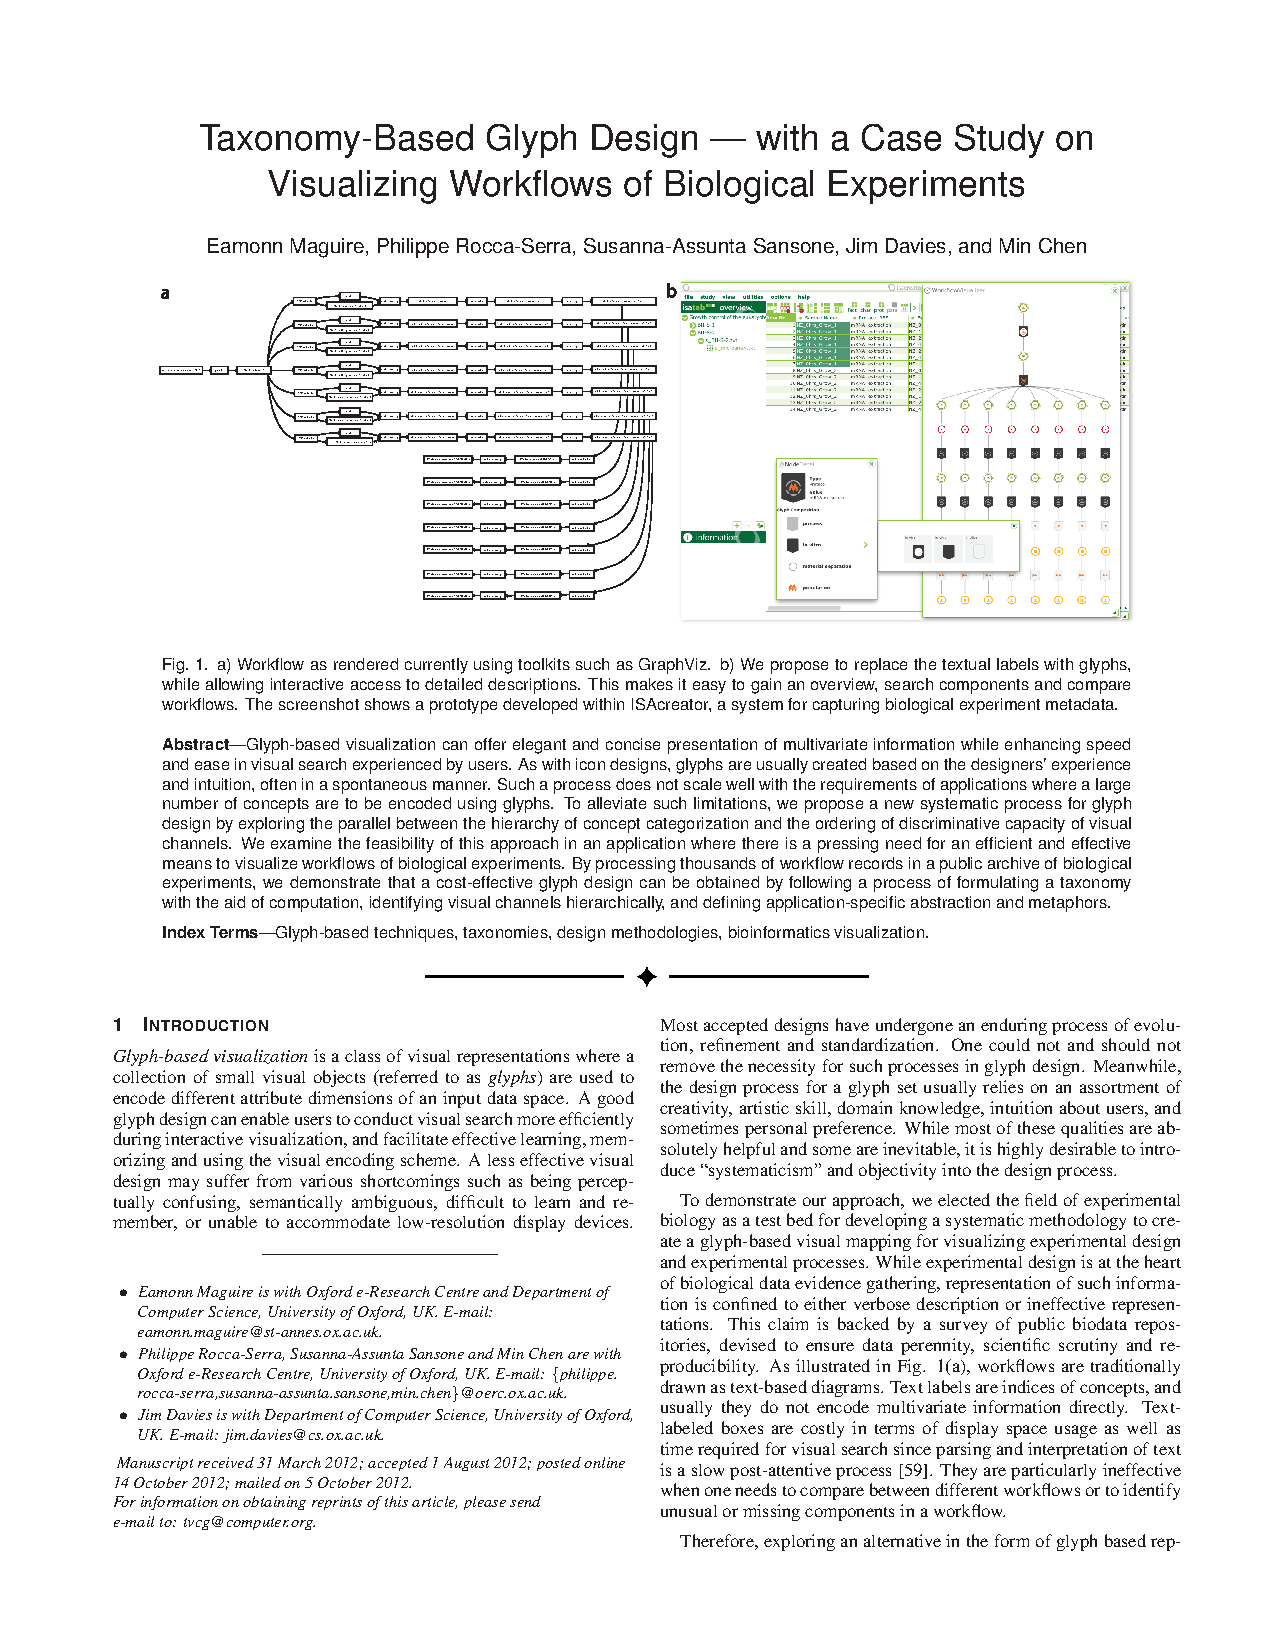
\includepdf[pages=-,pagecommand=\thispagestyle{plain}]{attachments/Taxonomy-basedGlyphDesign.pdf}

\section{Copy of \cite{Borgo:2013:EG}:\\~\\~\\Glyph-based Visualization: Foundations, Design Guidelines, Techniques and Applications}\label{app:star13}
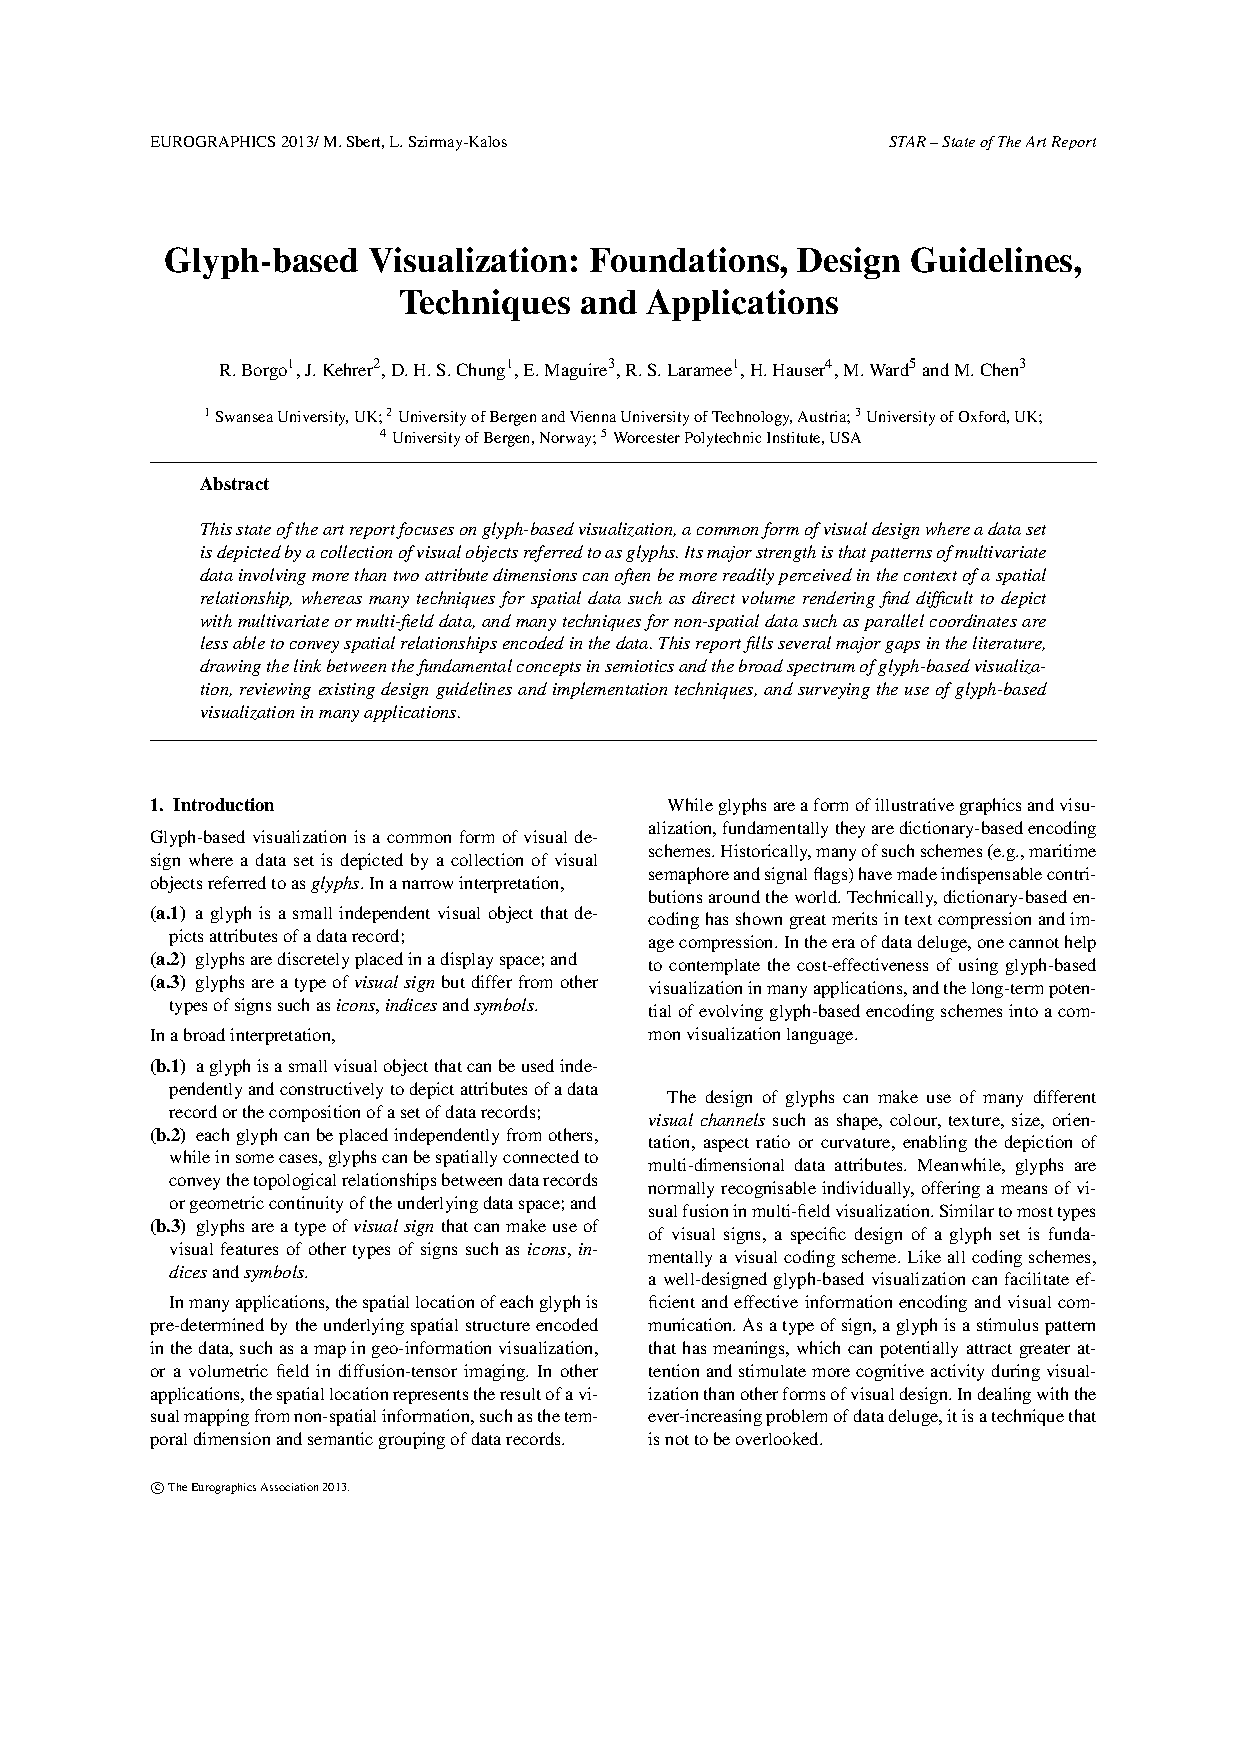
\includepdf[pages=-,pagecommand=\thispagestyle{plain}]{attachments/Borgo13GlyphBased.pdf}

\section{Copy of \cite{CGF:Abd2013a}:\\~\\~\\Rule-based Visual Mappings -- with a Case Study on Poetry Visualization}\label{app:poem13}
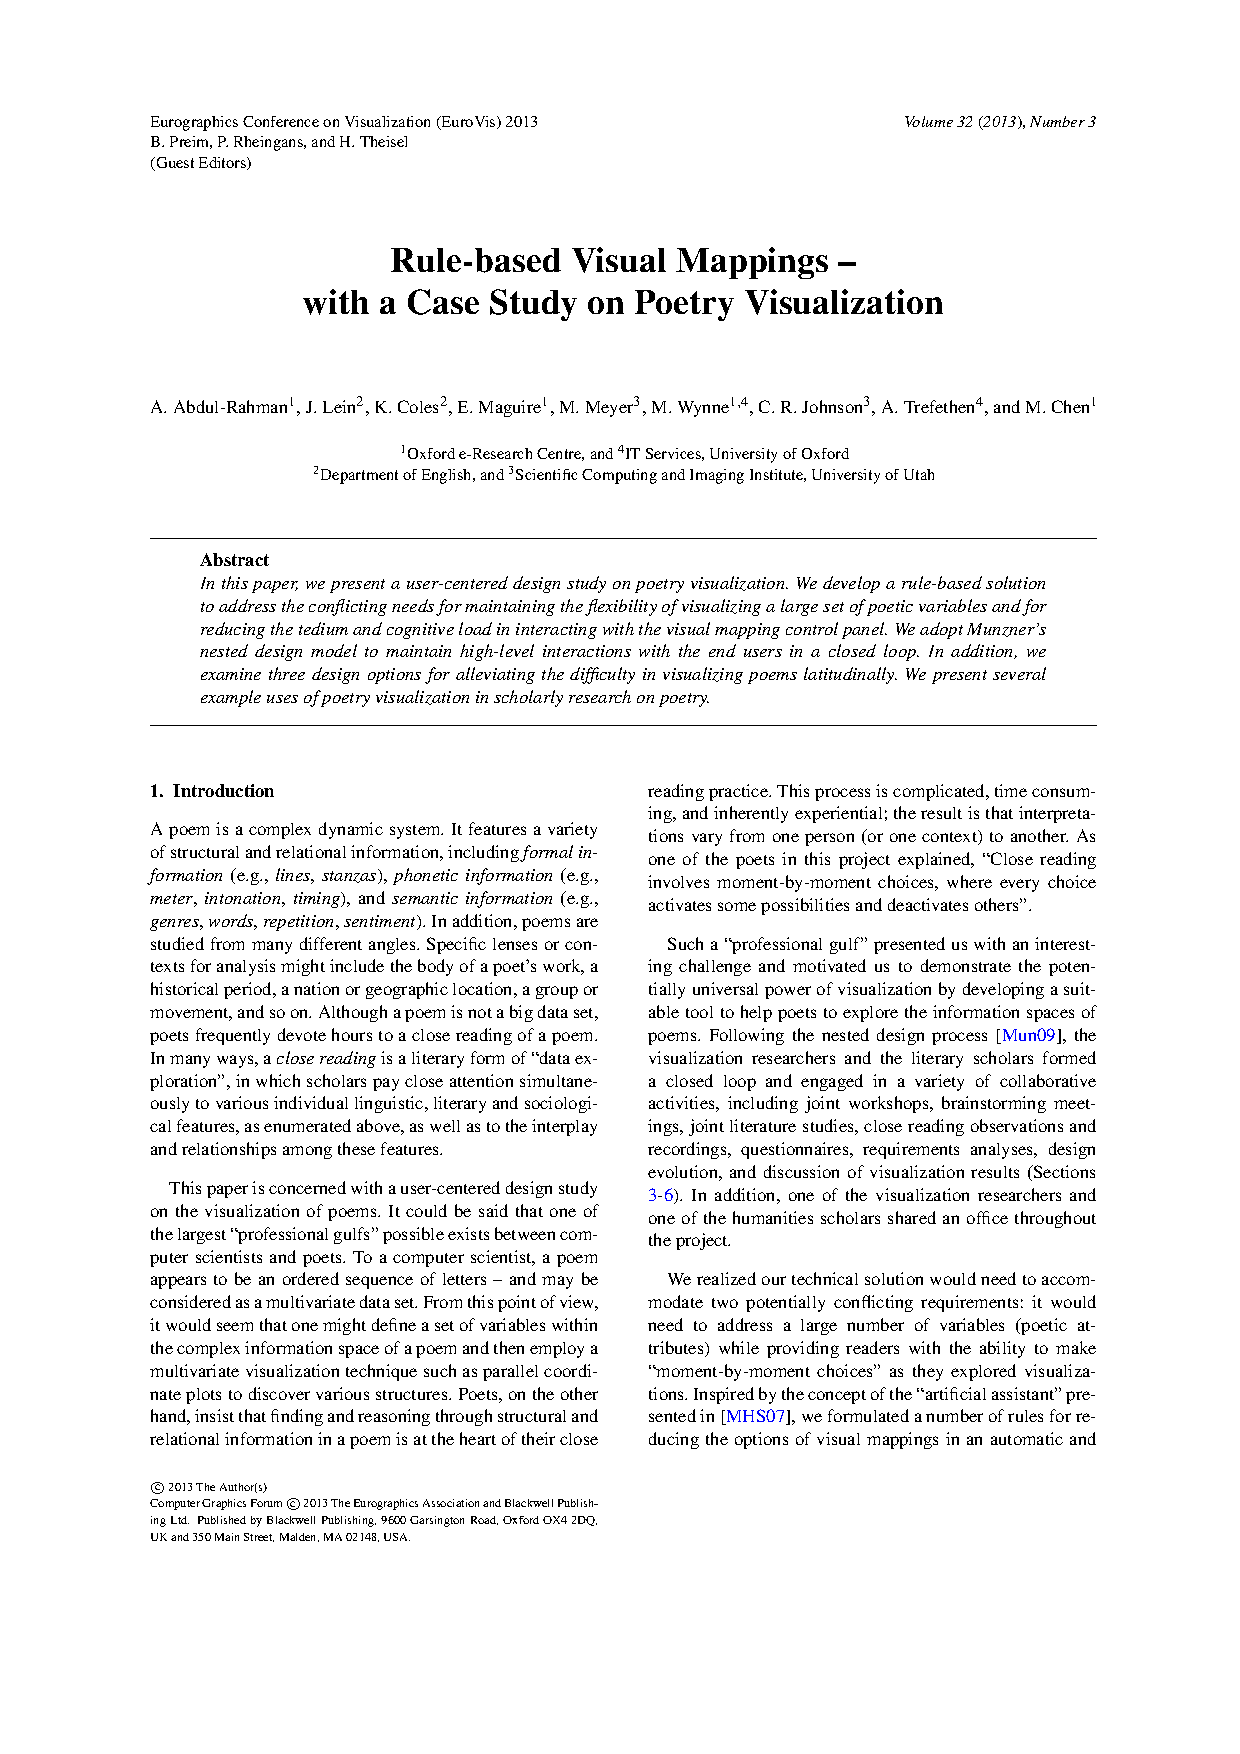
\includepdf[pages=-,pagecommand=\thispagestyle{plain}]{attachments/poemViewer-eurovis13.pdf}

\section{Copy of \cite{maguire13}:\\~\\~\\Visual Compression of Workflow Visualizations with Automated Detection of Macro Motifs}\label{app:ieee2013}
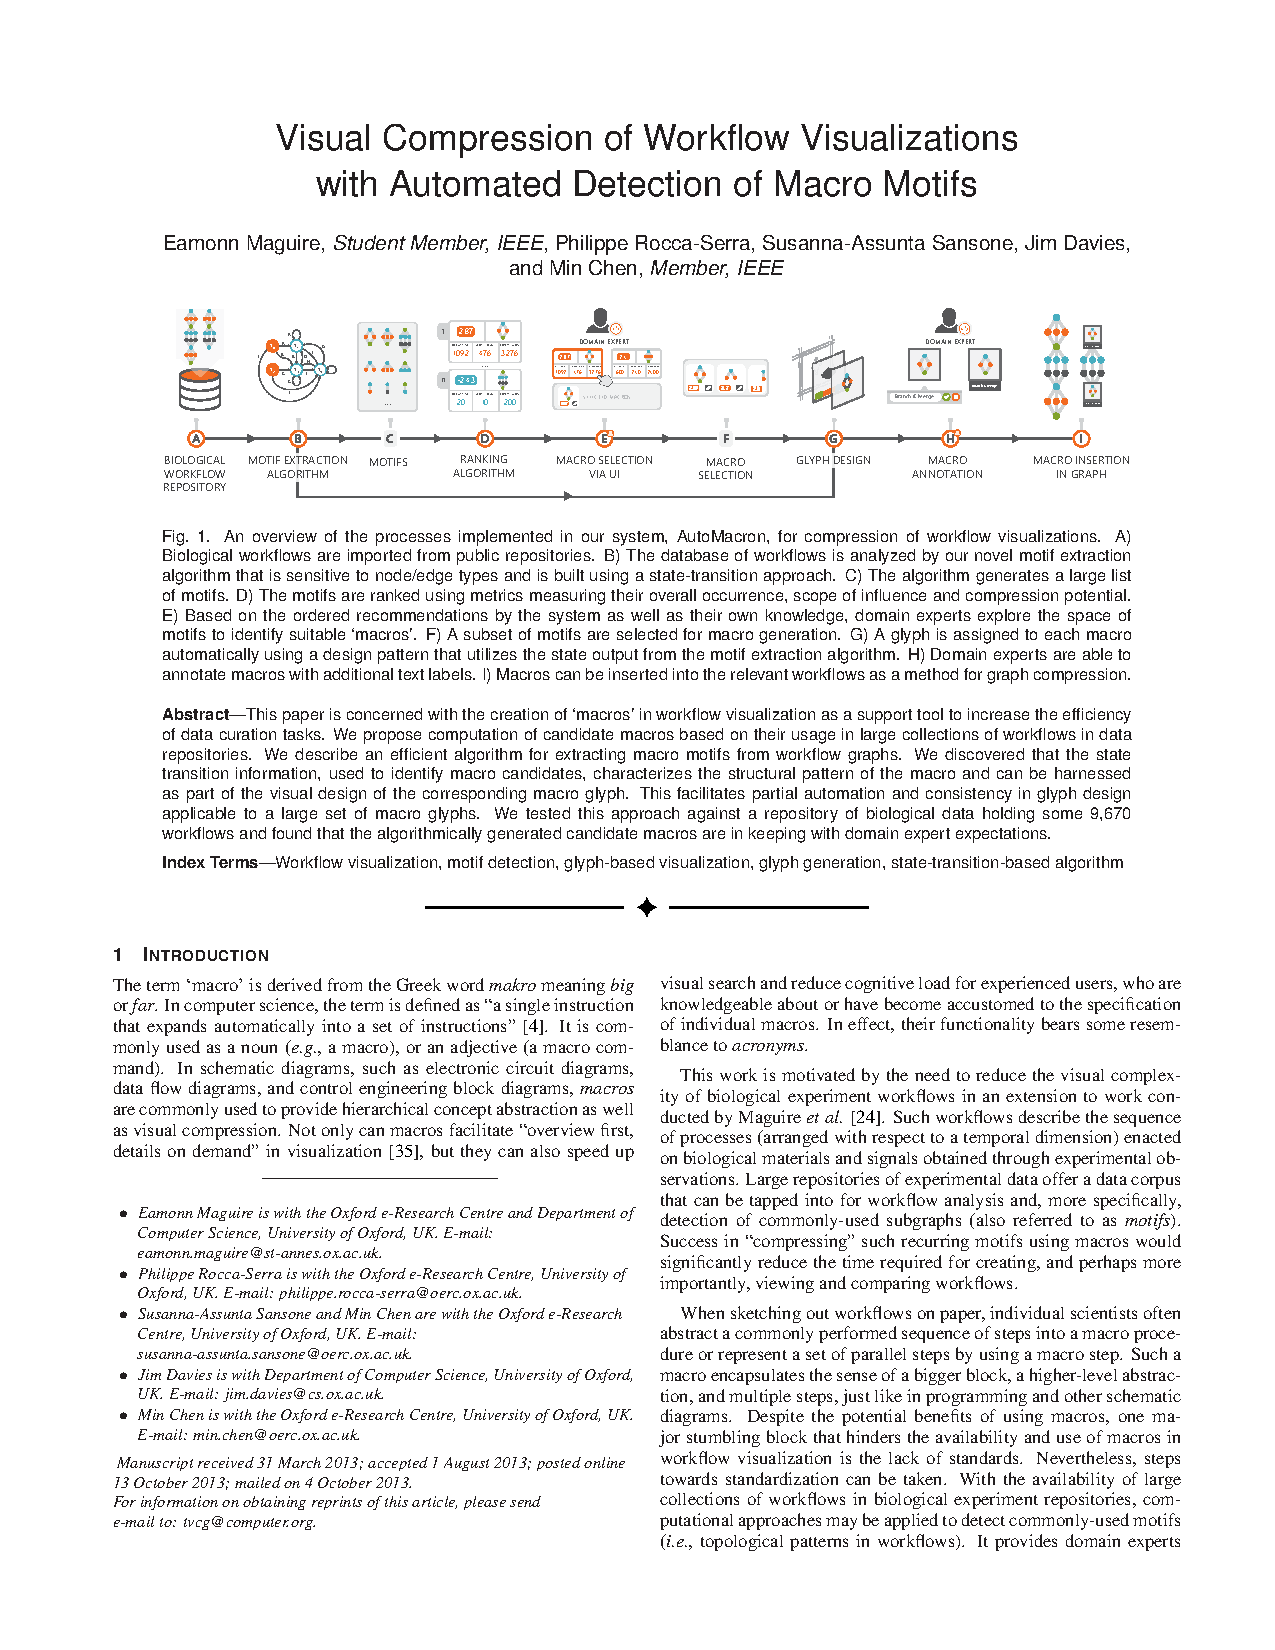
\includepdf[pages=-,pagecommand=\thispagestyle{plain}]{attachments/AutoMacron.pdf}

\section{Copy of \cite{CGF:maguire14-sp}:\\~\\~\\Redesigning the Sequence Logo with Glyph-based Approaches to Aid Interpretation}\label{app:eurovis-sp-14}
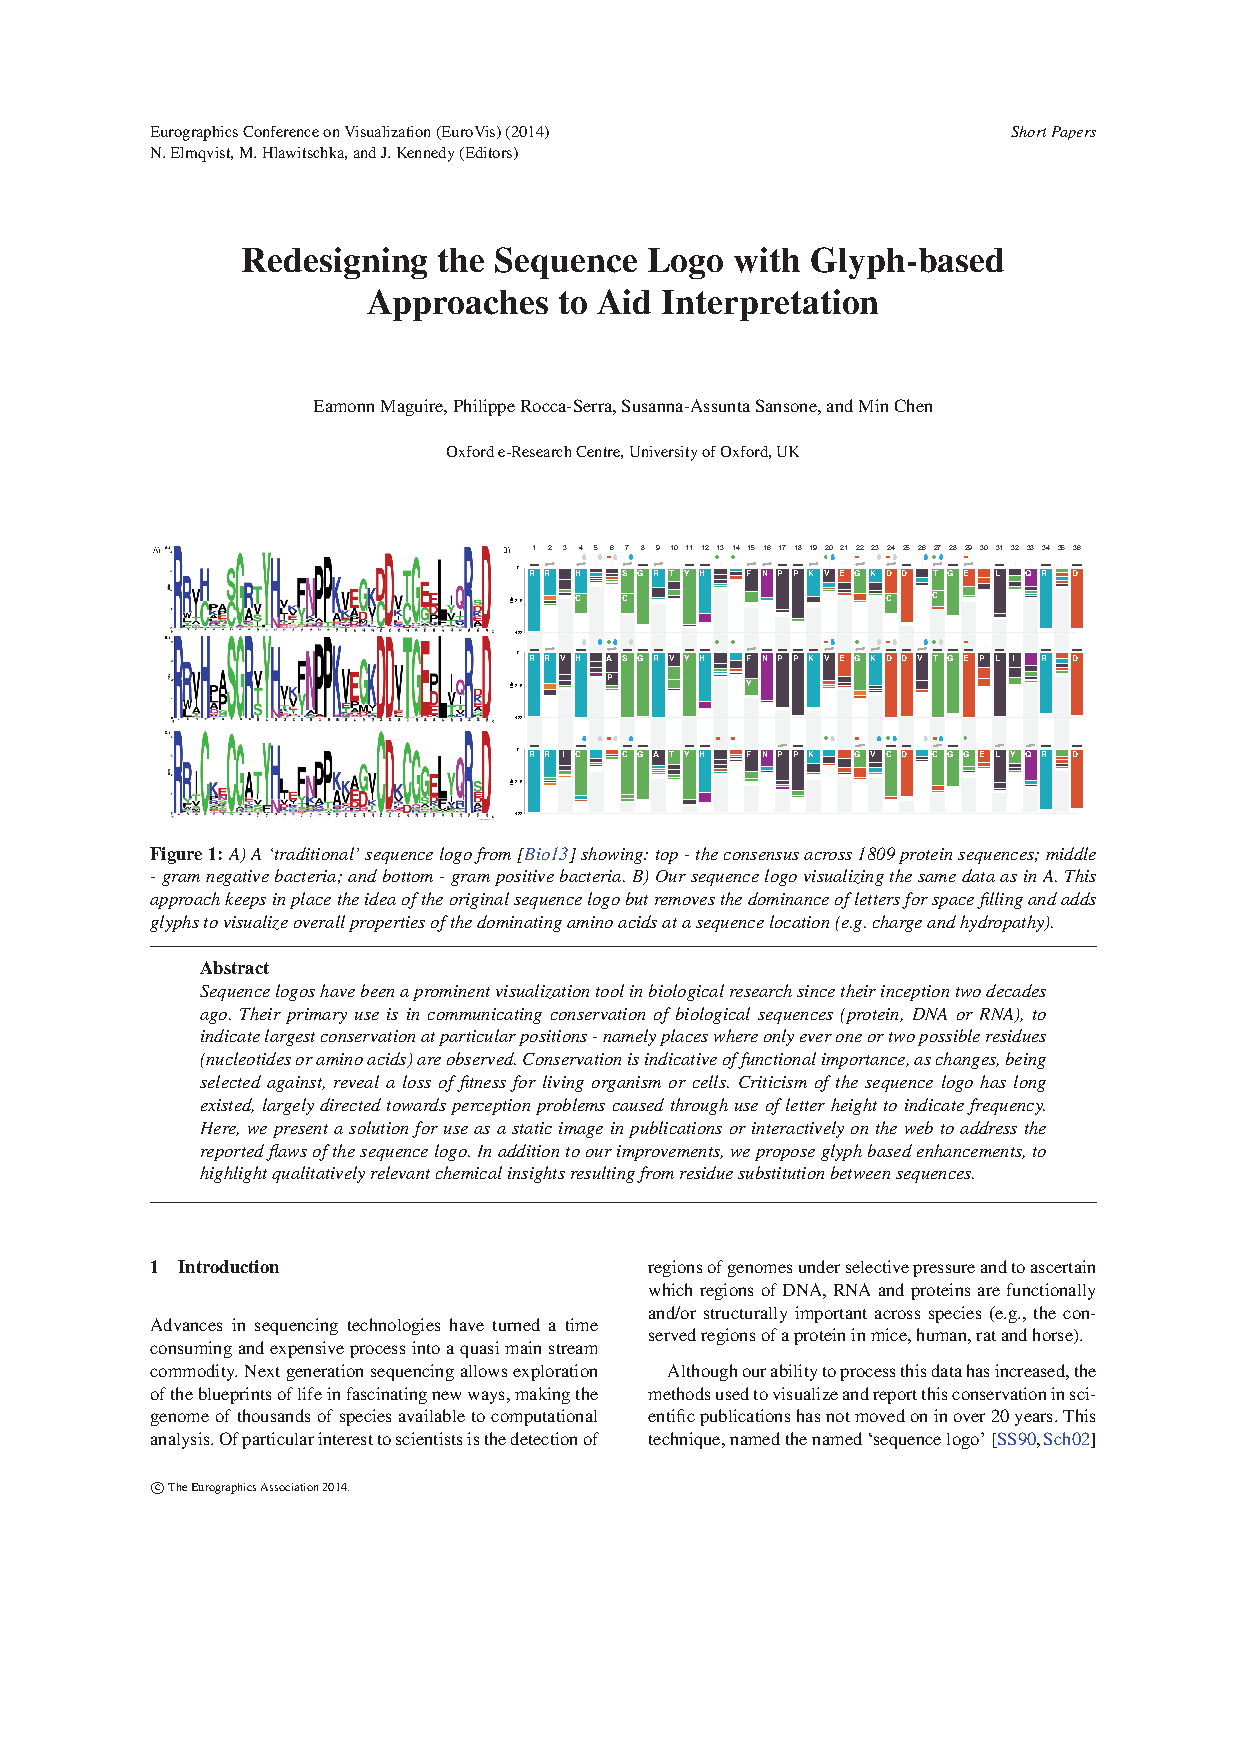
\includepdf[pages=-,pagecommand=\thispagestyle{plain}]{attachments/SequenceLogoRedesign.pdf}

\section{Copy of \cite{CGF:abdul-rahman14-sp}:\\~\\~\\Comparing Three Designs of Macro-Glyphs for Poetry Visualization}\label{app:eurovis-poem-sp-14}
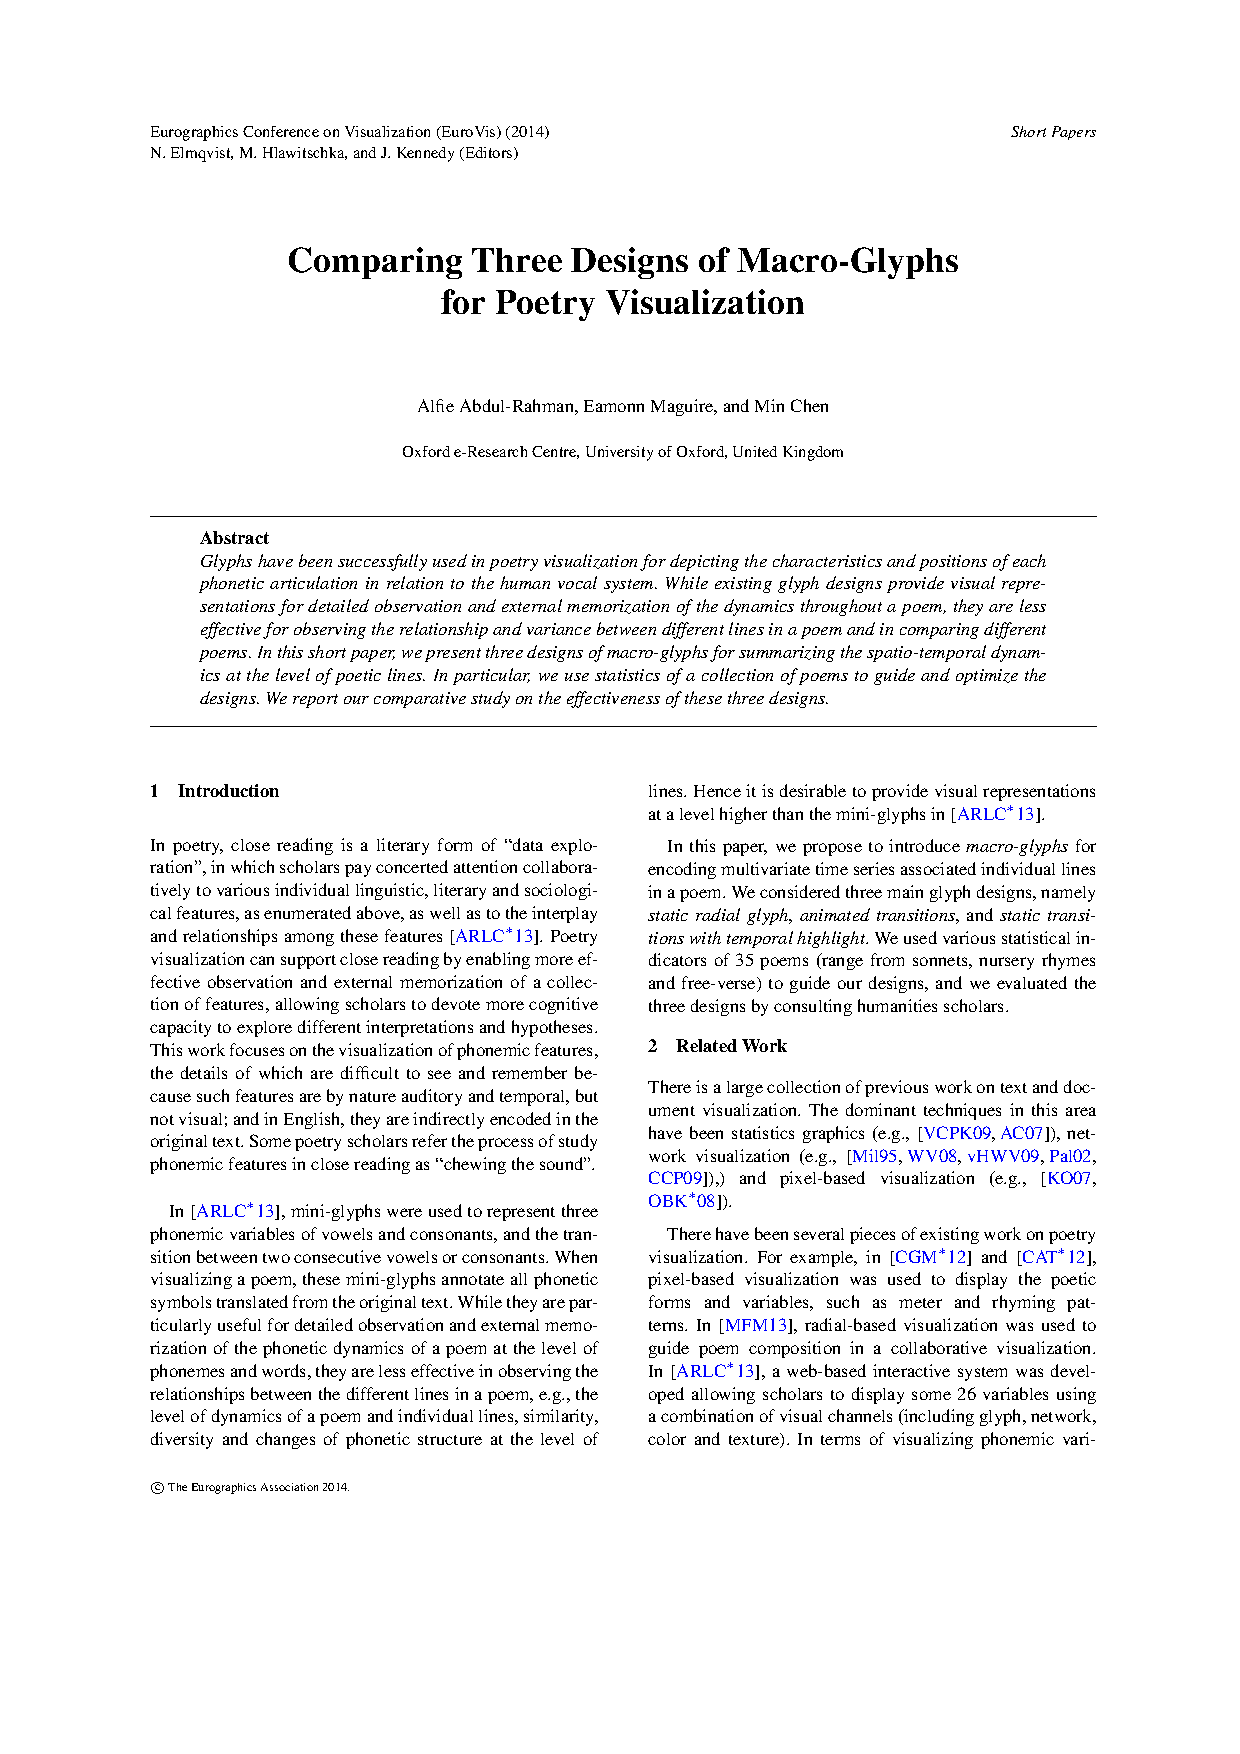
\includepdf[pages=-,pagecommand=\thispagestyle{plain}]{attachments/poem-shortpaper.pdf}

\section{Copy of \cite{legg14}:\\~\\~\\Fail-safe Glyph Encoding based on Quasi-Hamming Distances: With a Case Study on Visualizing File System Events}\label{app:legg-14}
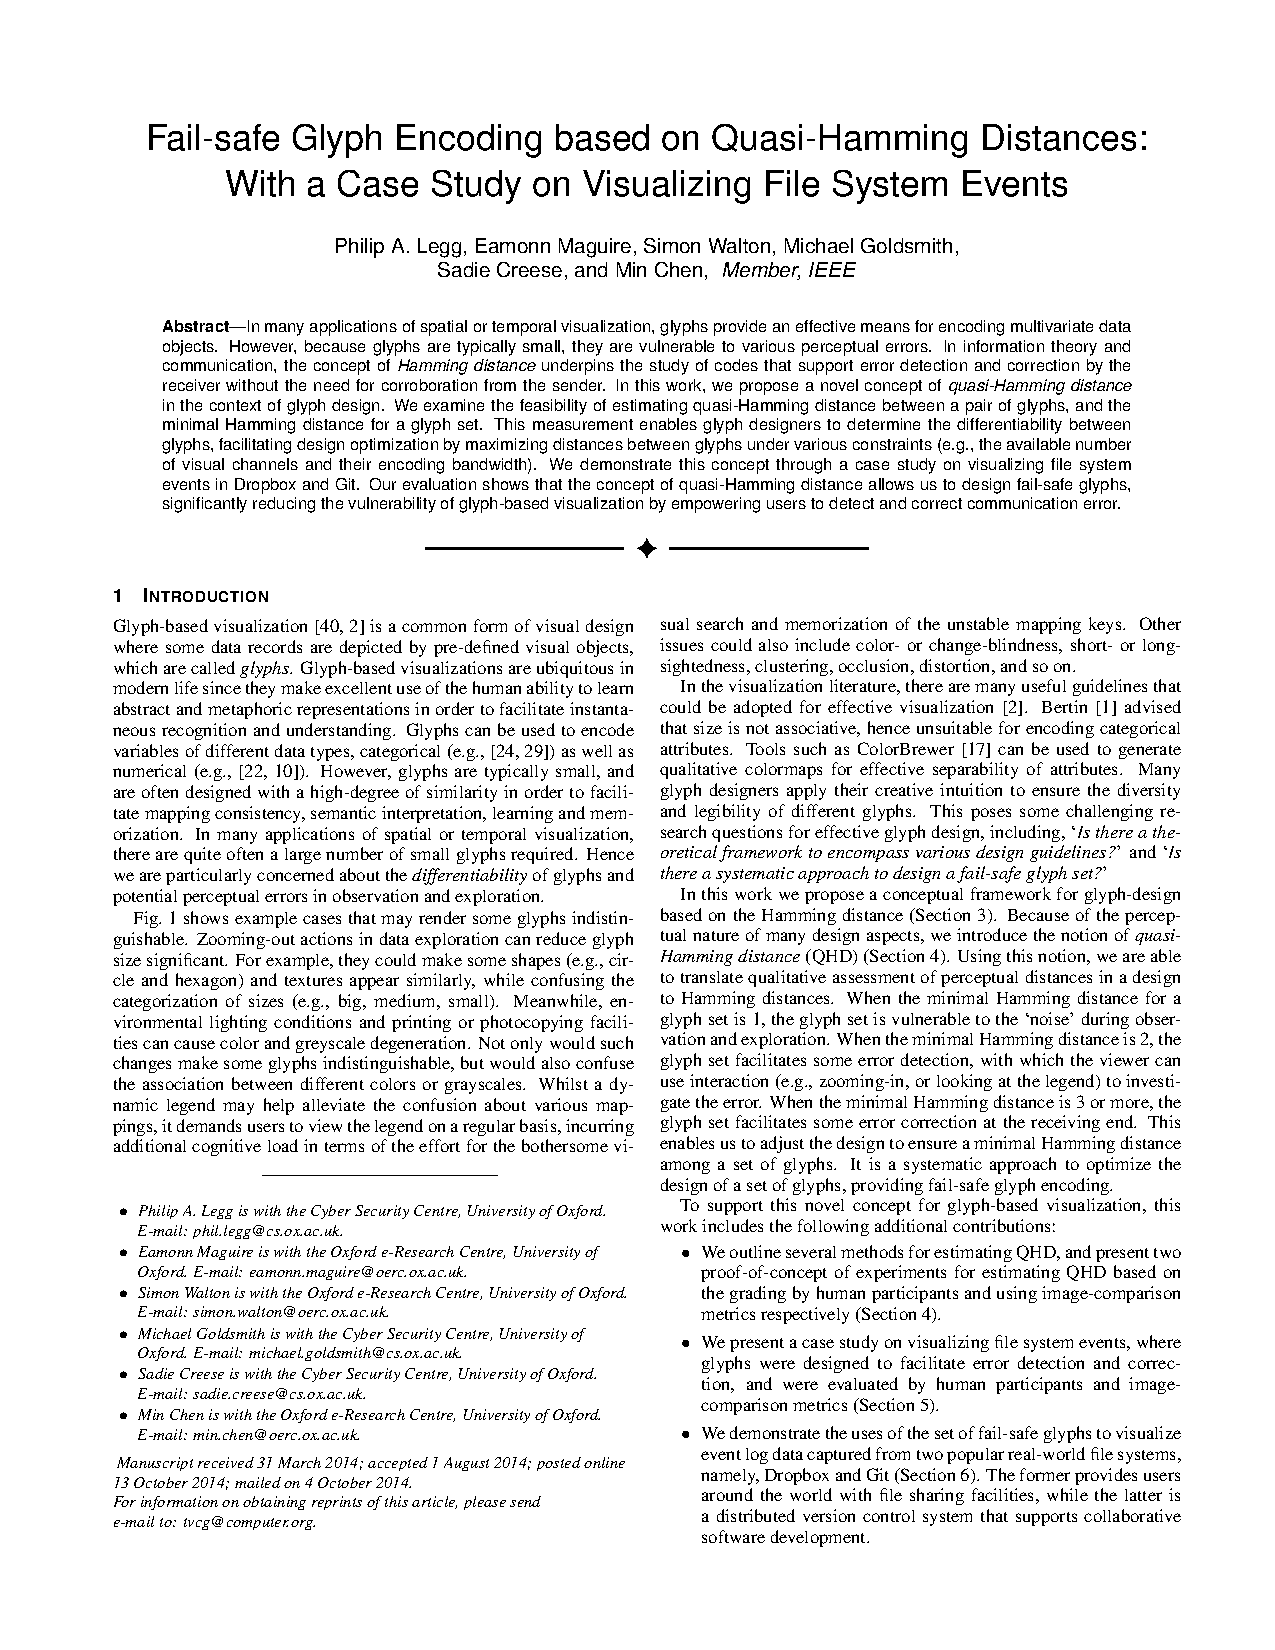
\includepdf[pages=-,pagecommand=\thispagestyle{plain}]{attachments/IEEE2014_failsafe_revised_v2.pdf}

\section{Copy of \cite{maguire14}:\\~\\~\\A Visual Analytical Approach for Model Editing and Testing in Glyph-based Time Series Compression}\label{app:ieee-14}
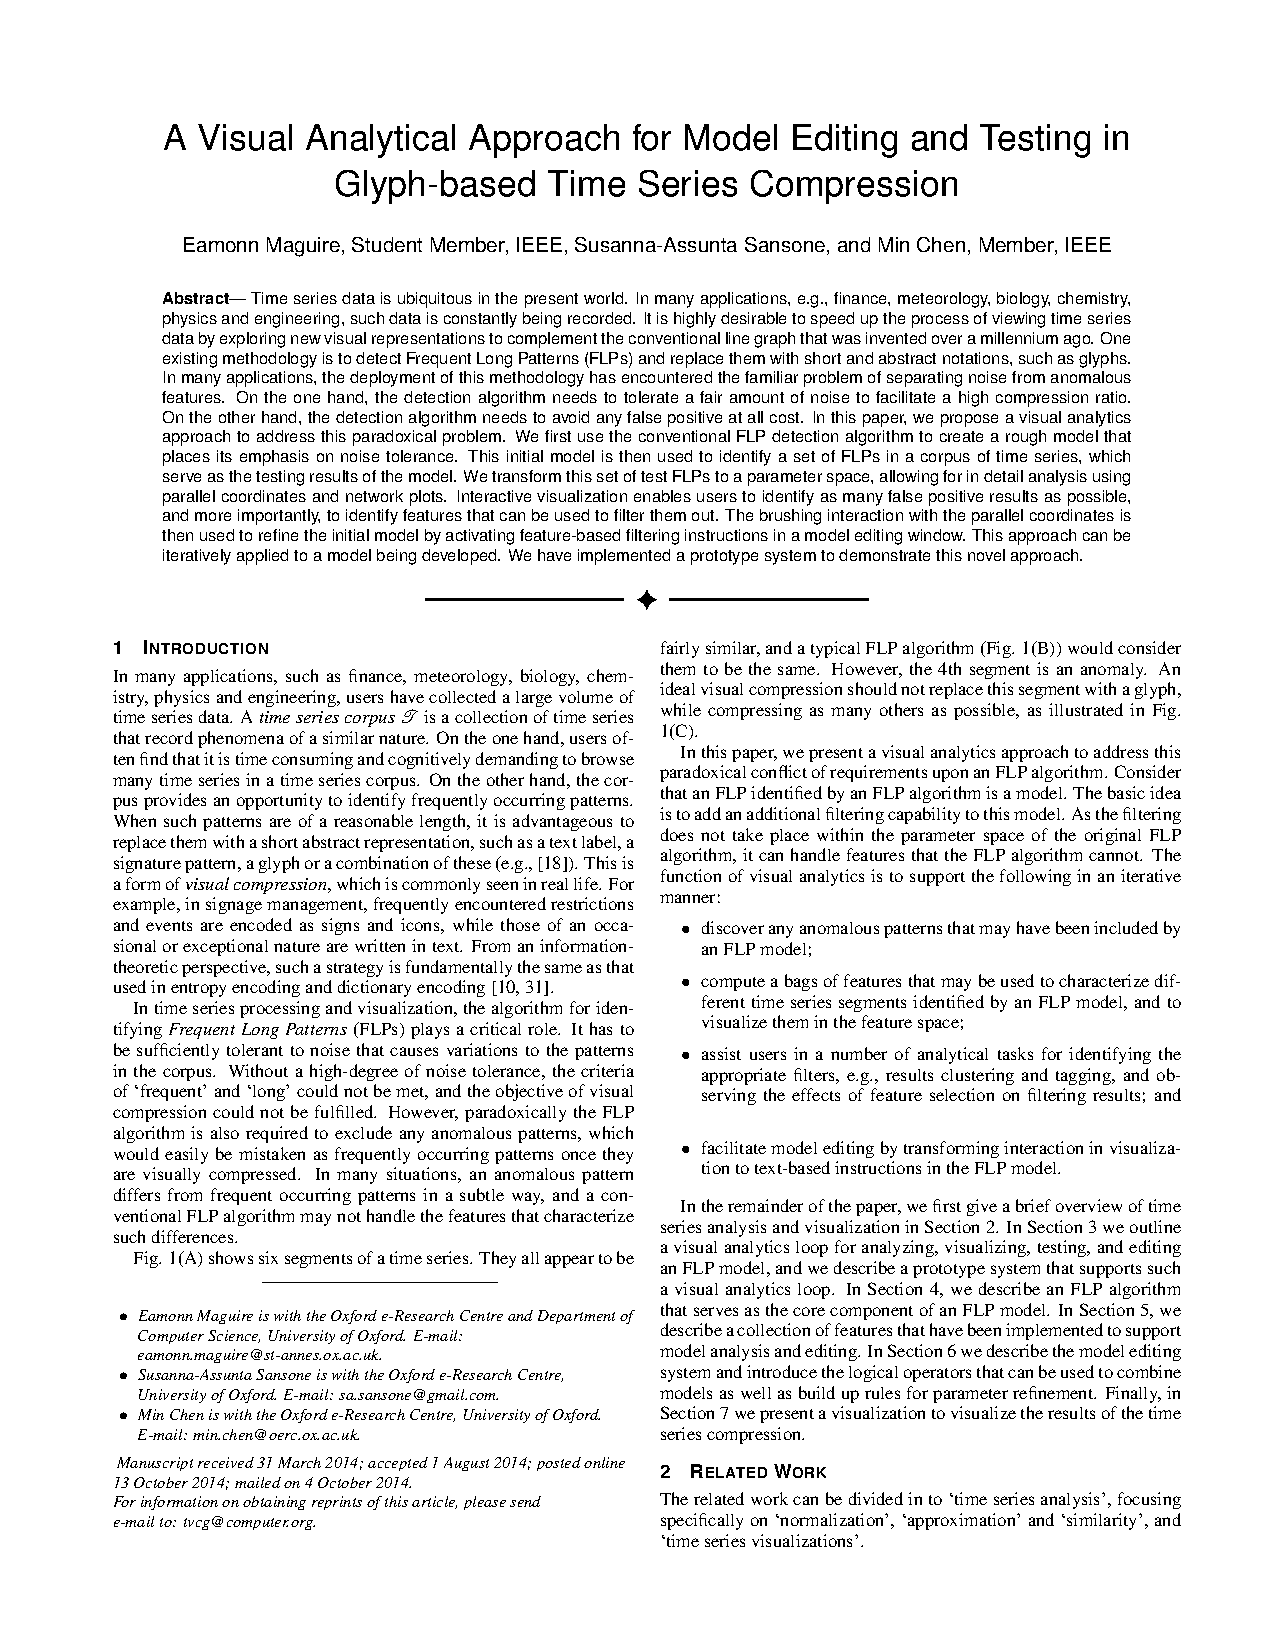
\includepdf[pages=-,pagecommand=\thispagestyle{plain}]{attachments/IEEE2014_Chronoglyph.pdf}

\end{document}
